% Credit:
% https://tex.stackexchange.com/questions/6534/is-there-a-package-to-create-optical-mark-reader-answer-sheets
\documentclass{article}
\usepackage{tikz}
\usepackage{tcolorbox}

\begin{document}

\begin{center}
\begin{tcolorbox}[width=5cm,
    standard jigsaw,
    opacityback=0]

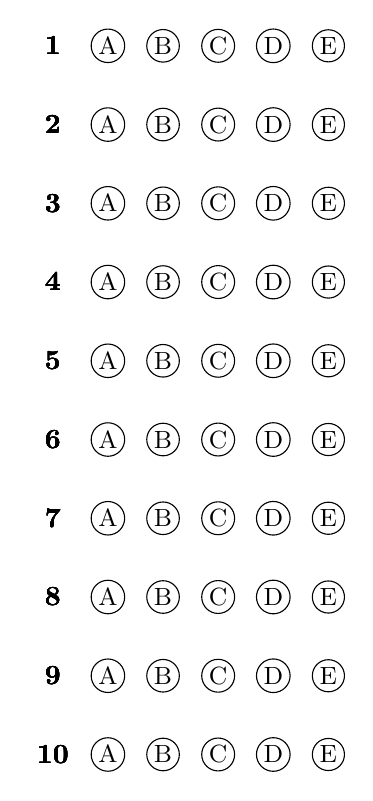
\begin{tikzpicture}[font=\small]
    \foreach \line in {1,2,...,10} {
        \begin{scope}[yshift=-\line cm]
            \foreach \count/\desc in {1/A, 2/B, 3/C, 4/D, 5/E} {
                \node at (0,0) {\normalsize\textbf{\line}};
                \node[draw,circle,inner sep=1pt] at ({\count * 0.7},0) {\desc};
            }
        \end{scope}
    }
\end{tikzpicture}

\end{tcolorbox}
\end{center}

\end{document}
